\documentclass[tikz,border=8pt]{standalone}
\usepackage{amsmath}
\usepackage{tikz}
\usetikzlibrary{positioning,arrows.meta,shapes.geometric,fit,backgrounds,calc}
\usepackage{fontspec}
\setmainfont{Times New Roman}

\begin{document}
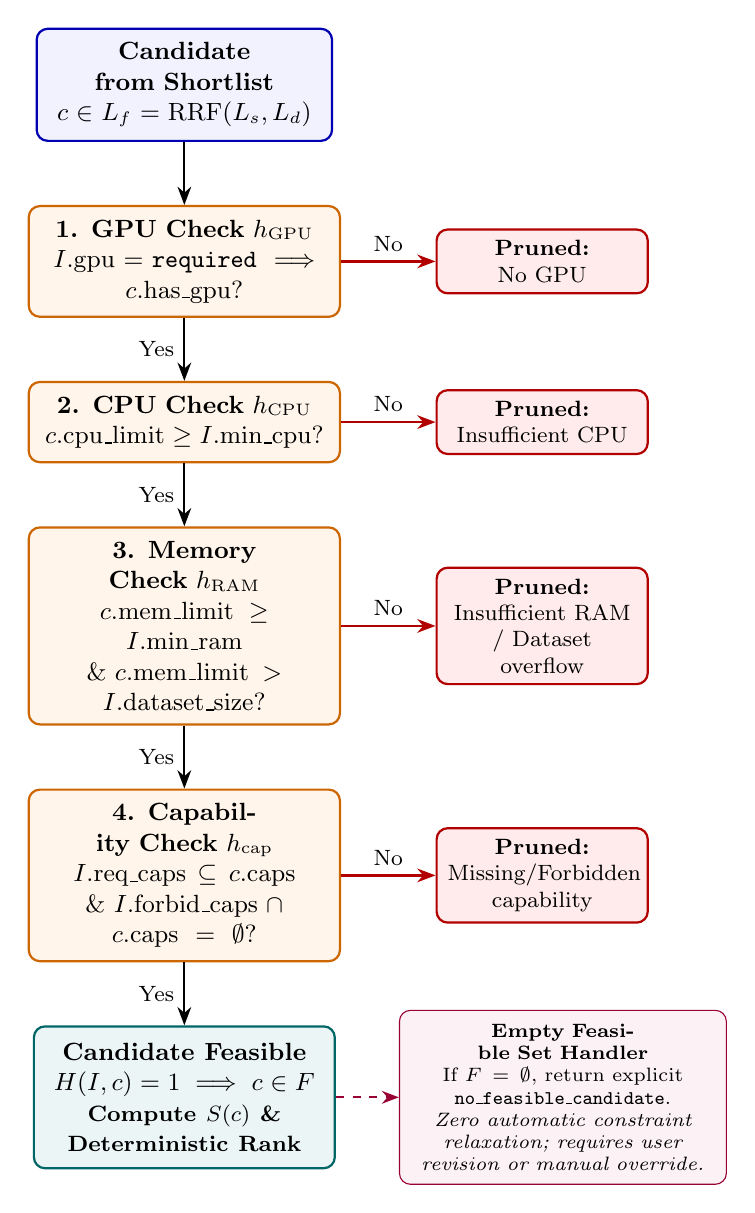
\begin{tikzpicture}[
    font=\small,
    >=Stealth,
    node distance=0.8cm and 1.2cm,
    stepbox/.style={
        draw=blue!70!black,
        fill=blue!5,
        rounded corners=4pt,
        align=center,
        line width=0.8pt,
        inner sep=5pt,
        text width=3.4cm,
        minimum height=0.8cm
    },
    decision/.style={
        draw=orange!80!black,
        fill=orange!8,
        rounded corners=4pt,
        align=center,
        line width=0.8pt,
        inner sep=5pt,
        text width=3.6cm,
        minimum height=0.85cm
    },
    pruned/.style={
        draw=red!70!black,
        fill=red!8,
        rounded corners=4pt,
        align=center,
        line width=0.8pt,
        inner sep=4pt,
        text width=2.4cm,
        font=\footnotesize
    },
    feasible/.style={
        draw=teal!80!black,
        fill=teal!8,
        rounded corners=4pt,
        align=center,
        line width=0.8pt,
        inner sep=6pt,
        text width=3.4cm,
        font=\small\bfseries
    }
]

% Start
\node[stepbox] (start) {\textbf{Candidate from Shortlist}\\$c \in L_f = \mathrm{RRF}(L_s, L_d)$};

% Constraints Chain
\node[decision, below=0.8cm of start] (gpu) {
    \textbf{1. GPU Check $h_{\mathrm{GPU}}$}\\
    $I.\mathrm{gpu} = \texttt{required} \implies c.\mathrm{has\_gpu}$?
};

\node[decision, below=0.8cm of gpu] (cpu) {
    \textbf{2. CPU Check $h_{\mathrm{CPU}}$}\\
    $c.\mathrm{cpu\_limit} \ge I.\mathrm{min\_cpu}$?
};

\node[decision, below=0.8cm of cpu] (ram) {
    \textbf{3. Memory Check $h_{\mathrm{RAM}}$}\\
    $c.\mathrm{mem\_limit} \ge I.\mathrm{min\_ram}$\\
    \& $c.\mathrm{mem\_limit} > I.\mathrm{dataset\_size}$?
};

\node[decision, below=0.8cm of ram] (caps) {
    \textbf{4. Capability Check $h_{\mathrm{cap}}$}\\
    $I.\mathrm{req\_caps} \subseteq c.\mathrm{caps}$\\
    \& $I.\mathrm{forbid\_caps} \cap c.\mathrm{caps} = \emptyset$?
};

% Feasible Node
\node[feasible, below=0.8cm of caps] (pass) {
    \textbf{Candidate Feasible}\\
    $H(I, c) = 1 \implies c \in F$\\
    \footnotesize Compute $S(c)$ \& Deterministic Rank
};

% Pruned Nodes (on right)
\node[pruned, right=1.2cm of gpu] (p_gpu) {\textbf{Pruned:}\\No GPU};
\node[pruned, right=1.2cm of cpu] (p_cpu) {\textbf{Pruned:}\\Insufficient CPU};
\node[pruned, right=1.2cm of ram] (p_ram) {\textbf{Pruned:}\\Insufficient RAM / Dataset overflow};
\node[pruned, right=1.2cm of caps] (p_caps) {\textbf{Pruned:}\\Missing/Forbidden capability};

% Connections Vertical (Pass)
\draw[->, line width=0.8pt] (start) -- (gpu);
\draw[->, line width=0.8pt] (gpu) -- (cpu) node[midway, left, font=\footnotesize] {Yes};
\draw[->, line width=0.8pt] (cpu) -- (ram) node[midway, left, font=\footnotesize] {Yes};
\draw[->, line width=0.8pt] (ram) -- (caps) node[midway, left, font=\footnotesize] {Yes};
\draw[->, line width=0.8pt] (caps) -- (pass) node[midway, left, font=\footnotesize] {Yes};

% Connections Horizontal (Fail)
\draw[->, line width=0.8pt, draw=red!70!black] (gpu) -- (p_gpu) node[midway, above, font=\footnotesize] {No};
\draw[->, line width=0.8pt, draw=red!70!black] (cpu) -- (p_cpu) node[midway, above, font=\footnotesize] {No};
\draw[->, line width=0.8pt, draw=red!70!black] (ram) -- (p_ram) node[midway, above, font=\footnotesize] {No};
\draw[->, line width=0.8pt, draw=red!70!black] (caps) -- (p_caps) node[midway, above, font=\footnotesize] {No};

% Empty Feasible Set Note
\node[draw=purple!80!black, fill=purple!5, rounded corners=4pt, text width=3.8cm, right=0.8cm of pass, align=center, font=\scriptsize, inner sep=5pt] (empty_note) {
    \textbf{Empty Feasible Set Handler}\\
    If $F = \emptyset$, return explicit\\
    \texttt{no\_feasible\_candidate}.\\
    \textit{Zero automatic constraint relaxation; requires user revision or manual override.}
};
\draw[->, line width=0.7pt, dashed, draw=purple!80!black] (pass) -- (empty_note);

\end{tikzpicture}
\end{document}
